\RequirePackage{luatex85}
\documentclass{standalone}

\usepackage{amsmath}

\usepackage{fontspec, unicode-math}
\setsansfont[Scale=MatchLowercase]{TeX Gyre Heros}
\setmathfont{TeX Gyre Termes Math}

\usepackage{tikz}
\usetikzlibrary{arrows.meta}
\usetikzlibrary{quotes}
\usetikzlibrary{positioning}

\tikzset{
  every picture/.style={font={\sffamily\normalsize}, >=stealth},
  every pin edge/.style={black}}

\begin{document}

  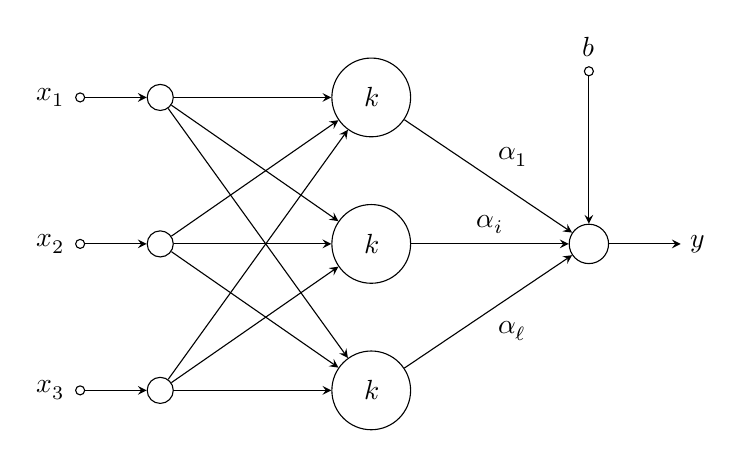
\begin{tikzpicture}[quotes mean pin, pin distance=6ex, node distance=0.5cm and 2cm,
    input/.style={draw, circle},
    kernel/.style={draw, circle, minimum size=1cm},
    output/.style={draw, circle, minimum size=0.5cm}]

    \begin{scope}[pin edge={<-{Circle[open]}}]
      \node[input] (IA) ["$x_{1}$" left] {};
      \node[input] (IB) ["$x_{2}$" left, below=10ex of IA] {};
      \node[input] (IC) ["$x_{3}$" left, below=10ex of IB] {};
    \end{scope}

    \node[kernel] (KA) [right=of IA] {$k$};
    \node[kernel] (KB) [right=of IB] {$k$};
    \node[kernel] (KC) [right=of IC] {$k$};

    \begin{scope}
      \node[output] (OP) [right=of KB,
        pin={[pin edge={<-{Circle[open]}}, pin distance=2cm]$b$},
        pin={[pin edge={->}]right:$y$}] {};
    \end{scope}

    \path[->] (IA) edge (KA) edge (KB) edge (KC);
    \path[->] (IB) edge (KA) edge (KB) edge (KC);
    \path[->] (IC) edge (KA) edge (KB) edge (KC);

    \path[->] (KA) edge["$\alpha_{1}$"] (OP);
    \path[->] (KB) edge["$\alpha_{i}$"] (OP);
    \path[->] (KC) edge["$\alpha_{\ell}$"'] (OP);
  \end{tikzpicture}

\end{document}
